%
% error.tex
%
\renewcommand{\thisname}{Chart::ErrorBars}
\section{\thisname}
\name{\thisname}
\file{ErrorBars.pm}
\requires{Chart::Base, GD, Carp, FileHandle}

\begin{Description}
The class \thisclass creates a point chart with error bars. This
class expects the error values within the data array. By use of the
\methoduse{add\_dataset()} method the error values are the next two sets
after the $y$ values. The first set after the $y$ values has to be the
set of values for the upper error bounds. The next set is the array of
the lower error bounds. Note that the error values are not specified
absolutely but rather as offsets from the $y$ value: the upper error
values will be added to the $y$ values, the lower error values will be
subtracted.

If you want to use the same value for the upper and lower error, you
can set the \attruse{same\_error} option to \literal{true}. In this
case only the set after the $y$ values is interpreted as a set of
errors.

Of course, it is also possible to use the \methoduse{add\_pt()}
method in the appropriate way to achieve the same results.
\thisclass is a subclass of \class{Chart::Base}.
\end{Description}

\example
\begin{figure}[ht]
  \begin{center}
    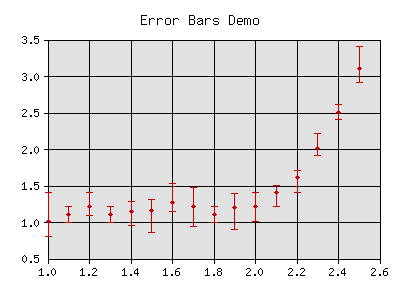
\includegraphics[scale=0.7]{error.png}
  \end{center}
  \caption{Error bars chart}
  \label{fig:error}
\end{figure}

\begin{verbatim}
use Chart::ErrorBars;
$g = Chart::ErrorBars->new();

# the x values
$g->add_dataset(qw(1    1.1  1.2  1.3  1.4  1.5  1.6  1.7
                   1.8  1.9  2    2.1  2.2  2.3  2.4  2.5));
# the y values
$g->add_dataset(qw(1    1.1  1.2  1.1  1.14 1.15 1.26 1.2
                   1.1  1.19 1.2  1.4  1.6  2.0  2.5  3.1));
# the upper errors
$g->add_dataset(qw(0.4  0.1  0.2  0.1  0.14 0.15 0.26 0.27
                   0.1  0.19 0.2  0.1  0.1  0.2  0.1  0.3));
# the lower errors
$g->add_dataset(qw(0.2  0.11 0.12 0.11 0.2  0.3  0.12 0.27
                   0.11 0.3  0.2  0.2  0.2  0.1  0.1  0.2));

$g->set( 'xy_plot'    => 'true',
         'precision'  => 1,
         'pt_size'    => 10,
         'brush_size' => 2,
         'legend'     => 'none',
         'title'      => 'Error Bars Demo',
         'grid_lines' => 'true'
       );

$g->png("errorbars.png");
\end{verbatim}

\constructorblurb{\thisname}

\begin{AttrDecl}{brush\_size}
Sets the width of the lines in pixels. Default is 6.
\end{AttrDecl}

\begin{AttrDecl}{pt\_size}
Sets the radius of the points in pixels. Default is 18.
\end{AttrDecl}

\begin{AttrDecl}{same\_error}
Tells \thisclass that you want to use the same values for
upper and lower error bounds if set to \literal{true}. Then you have to
add just one set of error values. Defaults to \literal{false}.
\end{AttrDecl}

\begin{AttrDecl}{sort}
Sorts the data in ascending order if set to \literal{true}. Should be
set if the input data is not sorted. Defaults to \literal{false}.
\end{AttrDecl}

\attrdecl{xlabels}
\begin{AttrDecl}{xrange}
This pair of options allows arbitrary positioning of $x$ axis labels.
The two options must either both be specified or both be omitted.
\attruse{xlabels} is a reference to 2-element array. The first of the
elements is a nested (reference to an) array of strings that are the
labels. The second element is a nested (reference to an) array of
numbers that are the $x$ values at which the labels should be placed.
\attruse{xrange} is a 2-element array specifying the minimum and maximum
$x$ values on the axis. \Eg,
\begin{verbatim}
@labels = (['Jan', 'Feb', 'Mar'],
           [10,    40,    70   ]);
$chart->set(xlabels => \bs @labels,
            xrange  => [0, 100]
           );
\end{verbatim}
\end{AttrDecl}

\begin{AttrDecl}{xy\_plot}
Forces \thisclass to plot a $x$--$y$ graph if set to \literal{true},
\ie, to treat the $x$ axis as numeric. Very useful for plots of
mathematical functions. Defaults to \literal{false}.
\end{AttrDecl}

\begin{AttrDecl}{y\_axes}
Tells \thisclass where to place the $y$ axis. Valid values are
\literal{left}, \literal{right} and \literal{both}. Defaults to
\literal{left}.
\end{AttrDecl}
